\chapter{Algorytm detekcji przeszkód}
\label{cha:algorytm}

% warto zrobić analizę osobno dla "nie FPGA" oraz dla FPGA
% potem dobrze by było zebrać dane w jakąś tabelę dla zgrabnego porównania
% dalej model programowy, jakieś parametry, elementy itp. + przykładowe obrazki, wykresy, dane itp.

% Jak to zrobiłem i dlaczego tak Napisać o tym, że wybrałem metodę na podstawie tych dwóch prac, dobierając kolejne elementy algorytmu, tak żeby jak najlpeiej rozwiązać ten problem. Zalażało mi na prostocie i możliwie niskiej złożoności obliczeniowej, żeby ułatwić implementacje na platformach wbudowanych
% Potem wymienienie etapów algorytmu - bardzo krótko bez opisu

% Dlaczego tradycyjny algorytm, a nie sieć neuronowa
Celem tego etapu projektu było zaprojektowanie, zaimplementowanie w~języku programowania Python, a~na koniec przetestowanie algorytmu detekcji przeszkód.

\vspace{11px}

Przyjęte założenia i cele:
\begin{enumerate}
    \item Algorytm powinien pozwalać na wykrywanie zarówno statycznych (względem układu odniesienia świata), jak i~poruszających się przeszkód.
    \item Powinien być możliwie nieskomplikowany obliczeniowo w celu zachowania możliwości późniejszej implementacji na wbudowanej platformie obliczeniowej. Ze względu na dużą ilość przetwarzanych danych, systemy wizyjne często charakteryzują się znaczną złożonością obliczeniową, dlatego warto projektować je tak, żeby ją ograniczyć.
    \item Musi dostarczać dane o obecności, położeniu i~odległości do przeszkody.
    \item Ma za zadanie wykrywać wiele obiektów znajdujących się w~polu widzenia kamery w~tym samym czasie.
\end{enumerate}

\section{Wybrane podejście}

W celu ułatwienia późniejszej implementacji na platformie wbudowanej, wszystkie podejścia bazujące na głębokich sieciach neuronowych zostały odrzucone. Algorytmy te charakteryzują się wysoką złożonością obliczeniową. Dla platform wbudowanych, które dysponują ograniczonymi zasobami, ich implementacja stanowi duże wyzwanie, szczególnie przy wymogu realizacji obliczeń w~czasie rzeczywistym.

% Taka decyzja została podjęta z~uwagi na trudność implementacji głębokich sieci neuronowych na platformie FPGA. Języki opisu sprzętu, w~jakich jest ona programowana, narzucają konieczność niskopoziomowej realizacji uczenia maszynowego. Podejście to znacznie różni się od tworzenia sieci neuronowych w~wysokopoziomowym języku programowania (Python), gdzie do dyspozycji użytkownika są rozbudowane, dedykowane biblioteki takie jak TensorFlow czy Pytorch.

% Wybrane prace

Podejście do rozwiązania problemu detekcji zostało przygotowane na podstawie analizy dwóch podobnych projektów, w~ramach których zaprojektowano zbliżone systemy: \cite{dynamic_obstacle} oraz \cite{night_obstacle}.

% Etapy algorytmu
\vspace{11px}
Algorytm wykrywania obiektów składa się z~następujących etapów:
\begin{enumerate}
    \item Odczyt i~akumulacja $N$ zdarzeń.
    \item Filtracja sygnału, w~celu eliminacji szumu tła (ang. \textit{background activity noise}).
    % \item Agregacja \textit{event'ów} do \textit{event frame'ów} w celu ich wizualizacji.
    \item Podział zdarzeń składających się na sygnał na klastry odpowiadające oddzielnym przeszkodom.
    \item Przypisanie do wykrytych obiektów indywidualnych identyfikatorów na podstawie algorytmu śledzącego ich ruch.
    \item Estymacja głębi dla każdej przeszkody za pomocą triangulacji oraz ustalenie ich pozycji w~trójwymiarowej przestrzeni.
\end{enumerate}

Wyjścia z~etapów pierwszego, drugiego i~czwartego, opcjonalnie mogą być wizualizowane, co ułatwiło przeprowadzanie testów.

% Grafikę ze schamtem działania można dać w sumie tu, albo w wynikach


Na rysunku \ref{fig:schemat} przedstawiono blokowy schemat działania systemu. Strzałkami zaznaczony jest przepływ danych między kolejnymi modułami (etapami) algorytmu. Na wejście podawany jest asynchroniczny strumień zdarzeń, a~na wyjściu otrzymywane są dane o~położeniu i~prędkości przeszkód. Dodatkowo odczytywać można obrazy wizualizujące przetwarzane dane na wyjściu wybranych etapów. Można je obserwować dzięki reprezentacji w~postaci ramek zdarzeniowych, realizowanych osobno przed i~po filtracji.

\begin{figure}
    \centering
    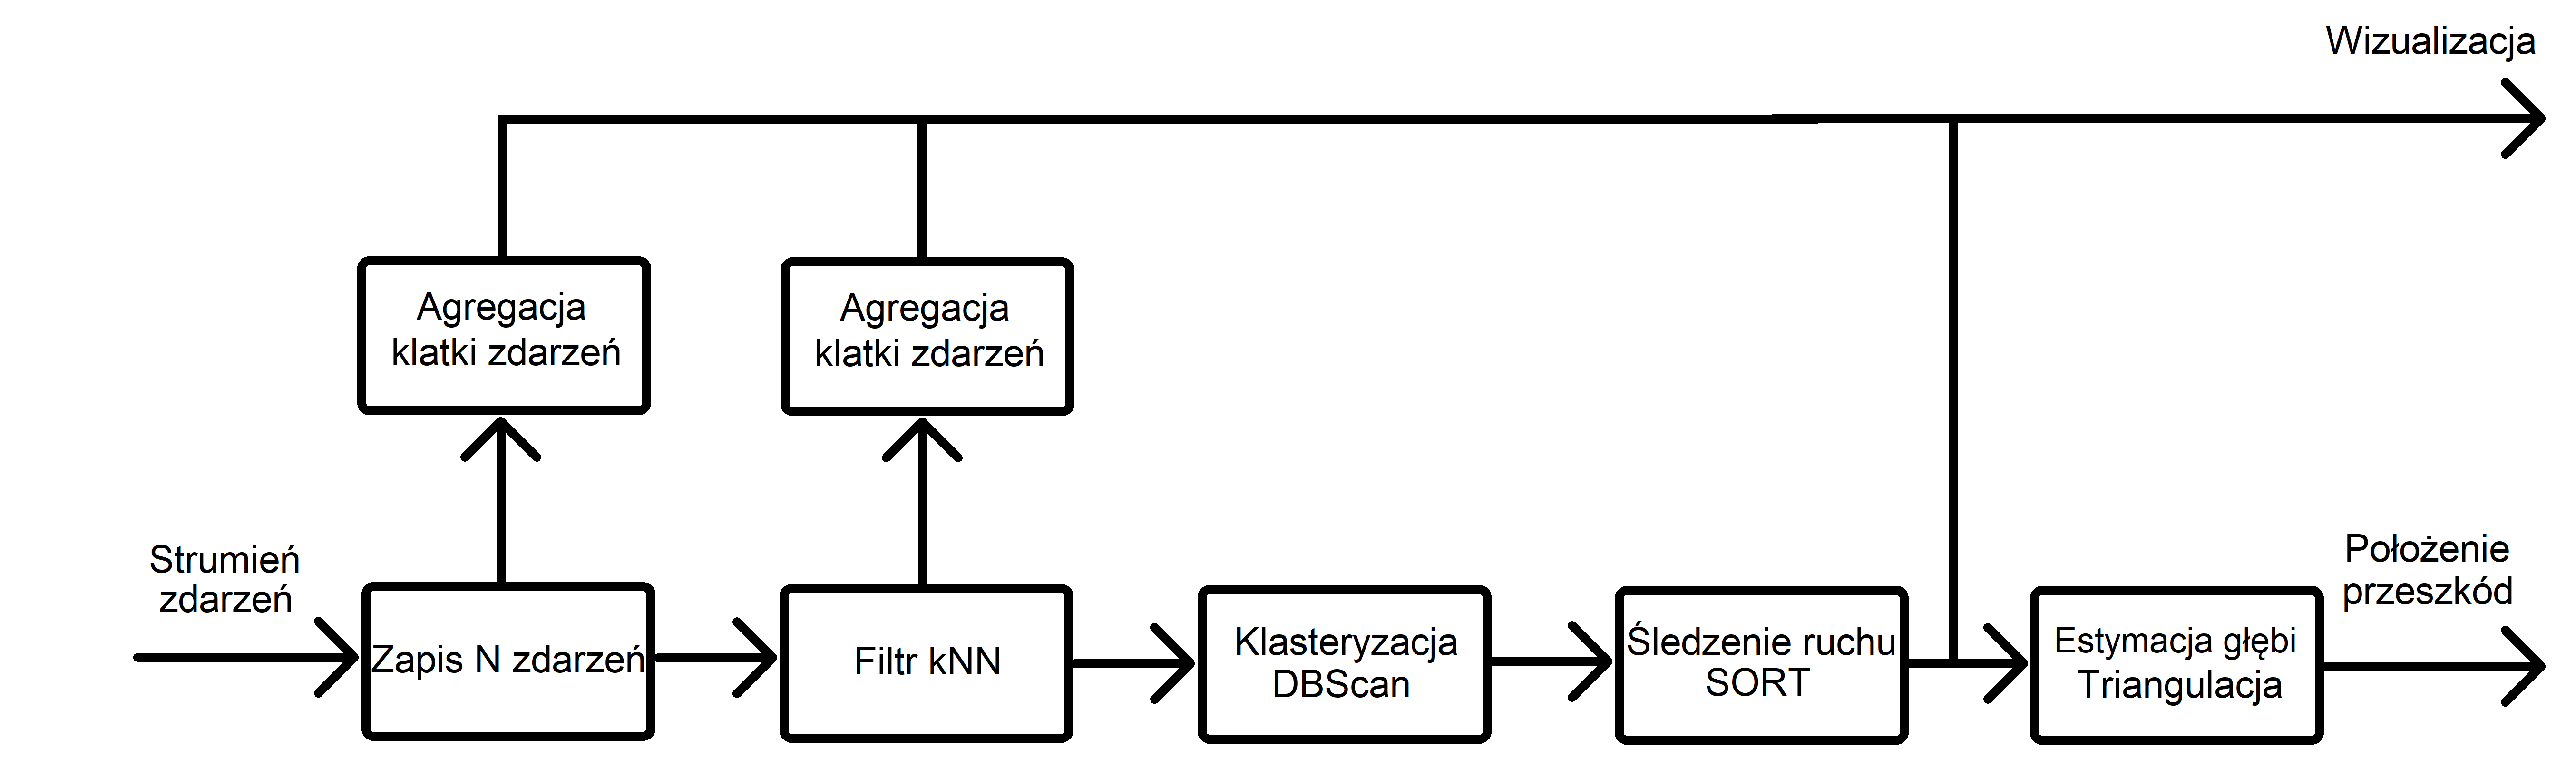
\includegraphics[width=1\linewidth]{images/schemat_detekcji.png}
    \caption{Schemat blokowy działania algorytmu.}
    \label{fig:schemat}
\end{figure}

\section{Implementacja}

% Wykorzystane narzędzia - język i biblioteki - sposób implementacji modelu programowego

% Dokładny opis po kolei każdego z etapów z listy - jak zrobiłem, jakie podejścia przetestowałem, jakich narzędzi użyłem

% \noindent \textbf{Podział eventów}
% \vspace{11px}
\subsection{Akumulacja zdarzeń}

% Żeby możliwe było wykrywanie przeszkód, otrzymywane w~asynchronicznym strumieniu zdarzenia nie mogą być przetwarzane pojedynczo
Aby móc wykorzystać otrzymywane w~asynchronicznym strumieniu zdarzenia do dalszej detekcji obiektów, najprostszym rozwiązaniem jest ich akumulacja i~zrzutowanie na płaszczyznę obrazu. Do tego zagadnienia można podejść na dwa sposoby:
\begin{itemize}
    \item Zbieranie zdarzeń z~określonego interwału czasowego. To intuicyjne rozwiązanie ma swoją wadę -- szczególnie jeśli czas akumulacji jest zbyt długi, na stworzonych za pomocą zgrupowanych w~ten sposób zdarzeń ramkach może być widoczne rozmycie ruchu szybko poruszających się obiektów. Można to zauważyć na rysunku \ref{fig:motion_blur}.
    
    \begin{figure}[H]
        \centering
        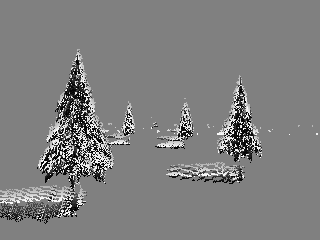
\includegraphics[width=0.4\linewidth]{images/motion_blur.png}
        \caption{Rozmycie ruchu widoczne, gdy czas odczytywania zdarzeń w celu ich podziału jest zbyt długi w stosunku do względnej prędkości obiektu.}
        \label{fig:motion_blur}
    \end{figure}
    
    \item Zbieranie $N$ zdarzeń -- ten sposób pozwala ograniczyć wspomniany problem, dlatego to on został wykorzystany. Wartość $N$ jest stała -- jest parametrem detektora, dla symulacji w Gazebo została ustawiona na $1500$. Jednak to rozwiązanie także ma swoją wadę -- w przypadku zbyt dużej dynamiki obiektów, gdy generowane jest dużo zdarzeń, wzrasta częstotliwość tworzenia nowych \textit{event frame}'ów, a wraz z nią spada liczba milisekund na ich przetworzenie przed pojawieniem się kolejnej ramki.
\end{itemize}

% \vspace{11px}
% \noindent \textbf{Filtracja sygnału}
% \vspace{11px}

\subsection{Filtracja sygnału}

Ponieważ w~danych z~rzeczywistych kamer zdarzeniowych często obecny jest szum, należy go usunąć, co zwiększy skuteczność algorytmu dzięki odrzuceniu fałszywych zdarzeń oraz zmniejszeniu ich ogólnej liczby.

Dokładne metody filtracji szumu kamer zdarzeniowych opisane są w~artykułach \cite{dba_filter} oraz \cite{denoising}.

W projekcie zastosowany został stosunkowo prosty, ale skuteczny algorytm kNN (ang. \textit{k-Nearest Neighbour}). Działa on według prostej zasady (rys. \ref{fig:kNN}). Jako sygnał uznawane są tylko te zdarzenia, w~których otoczeniu $n \times n$ w~czasie nie większym niż $t$ od chwili obecnej wystąpiło $k$ zdarzeń. Wartości $n$, $t$ oraz $k$ to parametry filtra. Dla symulatora zostały one dobrane eksperymentalnie i~ustawione jako:
$$n=3; ~~t=\frac{1}{60}s; ~~k=3$$

\begin{figure}
    \centering
    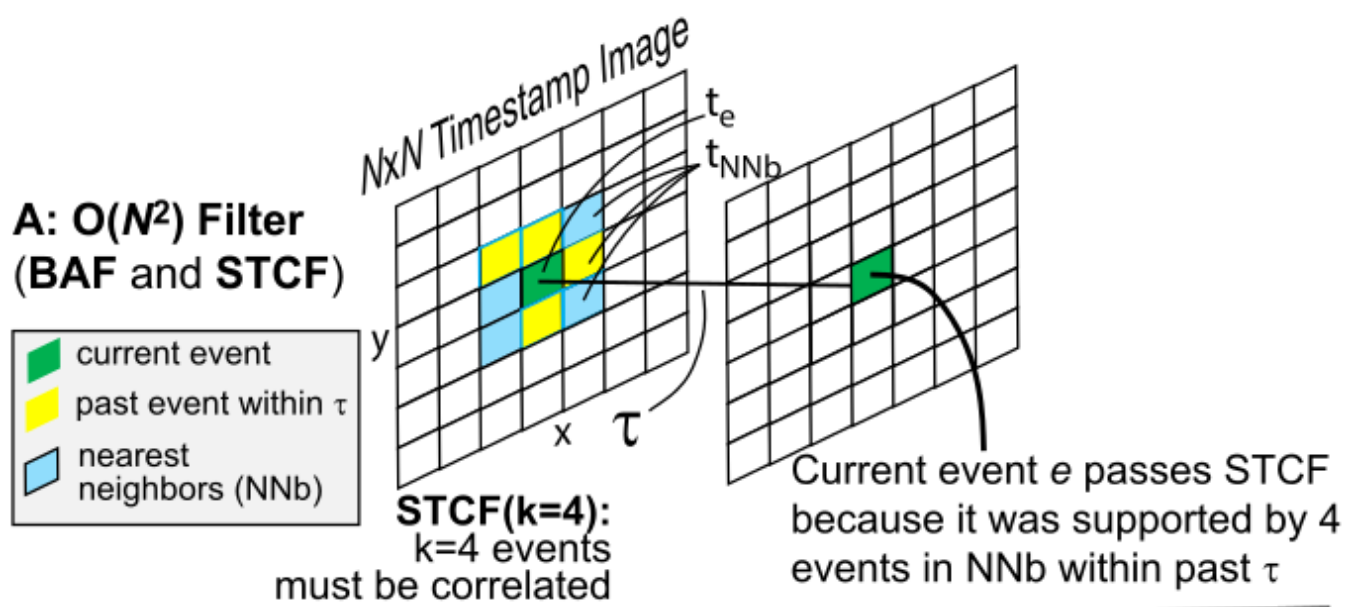
\includegraphics[width=0.7\linewidth]{images/kNN.png}
    \caption{Sposób działania filtra kNN. Źródło: \cite{denoising}.}
    \label{fig:kNN}
\end{figure}

Implementacja:
\begin{itemize}
    \item Tworzona jest macierz SAE (ang. \textit{Surface of Active Events}) o~rozmiarze obrazu, w~której przechowywany jest czas wystąpienia ostatniego zdarzenia dla każdego piksela,
    \item Dla każdego zdarzenia, podawanego na wejście detektora, sprawdzana jest odpowiednia dla niego ramka z~macierzy SAE i~liczeni są jego sąsiedzi,
    \item Jeśli jest ich co najmniej $k$, zdarzenie jest uznawany za poprawny, jeśli nie, jest odrzucany.
\end{itemize}

Zarówno oryginalne, jak i przefiltrowane zdarzenia, opcjonalnie mogą być zapisywane jako ramki zdarzeniowe w celu wizualizacji pracy algorytmu. Przykład wizualizacji zdarzeń po filtracji przedstawiony jest na rysunku \ref{fig:frame_example}.

\begin{figure}
    \centering
    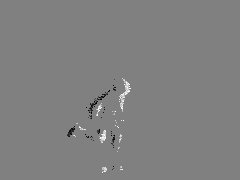
\includegraphics[width=0.4\linewidth]{images/filtered_run3.png}
    \caption{Przykład ramki zdarzeniowej uzyskanej z~danych ze zbioru \textit{night run} \cite{night_run}.}
    \label{fig:frame_example}
\end{figure}

% \vspace{11px}
% \noindent \textbf{Segmentacja na oddzielne obiekty}
% \vspace{11px}

\subsection{Segmentacja obiektów}

Celem tej fazy jest rozpoznanie w trójwymiarowej chmurze zdarzeń (wymiary: $x$, $y$ i $t$) odrębnych obiektów.

\vspace{11px}

W pierwszej kolejności do jego realizacji zostało wykorzystane podejście zaprezentowane w \cite{night_obstacle} -- dopasowywanie płaszczyzn za pomocą algorytmu RHT (ang. \textit{Randomised Hough Transform}) \cite{RHT}.

RHT to algorytm, który może być zastosowany do dopasowania równań (w tym przypadku równań płaszczyzn w postaci $ax + by + cz + d = 0$) do zbioru punktów. Bazuje on na transformacji Hougha, ale charakteryzuje się mniejszą złożonością obliczeniową. Ze zbioru punktów (tutaj zdarzeń, rozpatrywanych jako punkty w przestrzeni 3D o współrzędnych $t$, $x$ oraz $y$) losowo wybierane są trzy, dla których obliczane są parametry płaszczyzny. Jest to powtarzane wielokrotnie, a obliczane płaszczyzny akumulowane są w przestrzeni Hougha. Jest to taka przestrzeń, w której wymiarami są parametry równania $(a, b, c, d)$, w której dla każdego ich zestawu zliczana jest liczba jego wystąpień.
%Jest to powtarzane wielokrotnie, a~za każdym razem gdy płaszczyzna powtarza się, dodawany jest dla niej jeden głos.
Za dopasowane płaszczyzny uznawane są te, które zebrały najwięcej głosów (wystąpiły najwięcej razy).

Algorytm RHT został zaimplementowany w~Pythonie na podstawie artykułu \cite{RHT}. Następnie rozwiązanie to zostało przetestowane. Niestety, nie udało się osiągnąć żadnych zadowalających wyników spełniających zdefiniowany dla tej fazy cel. Mogło to być spowodowane trudnościami z~doborem parametrów algorytmu. Nie można też wykluczyć niewykrytych błędów w kodzie.

\vspace{11px}

RHT zastąpiono innym podejściem obecnym w~projekcie \cite{dynamic_obstacle}. Do przypisania zdarzeń do poszczególnych obiektów wykorzystywany jest algorytm do klasteryzacji DBScan \cite{DBScan}. Charakteryzuje się on kilkoma ważnymi zaletami:
\begin{itemize}
    \item Nie wymaga określenia z~góry liczby klastrów,
    \item Znajduje klastry o~dowolnym kształcie,
    \item Jest odporny na występowanie szumu,
    \item Jest zaimplementowany i~dostępny do wykorzystania w Pythonie w~bibliotece \textit{scikit-learn}.
\end{itemize}

DBScan ma dwa parametry wejściowe: $\epsilon$ -- maksymalny promień sąsiedztwa oraz $minP$ -- minimalną liczbę punktów wchodzących w skład klastra. Dla symulacji zostały one ustawione na:
$$\epsilon=7 ; ~~minP=30 $$

% W tym przypadku grupowanie zdarzeń okazało się działać w~pełni poprawnie. Poszczególne obiekty zapisywane są jako osobne przeszkody i~jako takie dalej przetwarzane.

% \vspace{11px}
% \noindent \textbf{Estymacja głębi}
% \vspace{11px}

% SORT
\subsection{Śledzenie obiektów}
\label{sec:tracking}

Kolejny etap (estymacja głębi) wymaga zapewnienia możliwości odczytywania informacji o~tej samej przeszkodzie, pochodzących z~obecnej i~z~poprzednich iteracji algorytmu. Taką opcję zapewnia zastosowanie narzędzia śledzącego ruch wykrytych obiektów -- SORT \cite{sort}. System ten na wejście przyjmuje detekcje obiektów w~postaci opisanych na nich prostokątów. Dla każdego przewiduje ruch, dzięki zastosowaniu modelu predykcji, wykorzystującego filtr Kalmana. Jest powszechnie używany do estymacji przyszłego stanu obiektu (np. prędkości, położenia) na podstawie obserwacji. Następnie dopasowuje wejściowe detekcje do wcześniej śledzonych obiektów. Zwraca ich położenie wraz z~przypisanym do niego indywidualnym numerem identyfikacyjnym. Dzięki temu do każdej wykrytej przeszkody przypisywany jest unikalny numer ID, co pozwala na dopasowanie do siebie obiektów między kolejnymi iteracjami algorytmu. Przykład działania algorytmu śledzenia obiektów widoczny jest na rysunku \ref{fig:tracking}.

\begin{figure}
    \centering
    \begin{minipage}{0.33\textwidth}
        \centering
        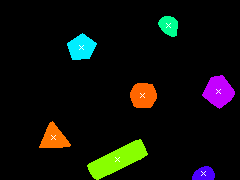
\includegraphics[width = 0.95\textwidth]{images/tracking1.png}
        \label{gra:tracking1}
    \end{minipage}\hfill
    \begin{minipage}{0.33\textwidth}
        \centering
        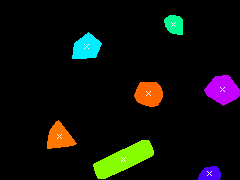
\includegraphics[width = 0.95\textwidth]{images/tracking2.png}
        \label{gra:tracking2}
    \end{minipage}\hfill
    \begin{minipage}{0.33\textwidth}
        \centering
        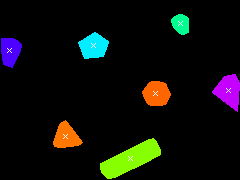
\includegraphics[width = 0.95\textwidth]{images/tracking3.png}
        \label{gra:tracking3}
    \end{minipage}
    \caption{Przeszkody wykryte w danych \textit{shapes rotation} w~trzech kolejnych iteracjach algorytmu. Widoczne kształty są efektem działania algorytmu klasteryzacji DBScan. Kolory, którymi zaznaczone są zajmowane przez obiekty obszary, są na stałe przypisane do indywidualnego ID każdej przeszkody. Na zestawianiu obrazków widoczny jest więc efekt działania algorytmu SORT -- obiekty są skutecznie śledzone.}
    \label{fig:tracking}
\end{figure}

Na tym etapie możliwa jest opcjonalna wizualizacja wykrytych obiektów.

\subsection{Estymacja głębi}

Obliczenie odległości wykrytego obiektu od drona jest ważnym elementem algorytmu, ponieważ pozwala na określenie pozycji przeszkody w~przestrzeni 3D.

W przypadku gdy zastosowany jest układ kamer stereo, zadanie to można wykonywać za pomocą triangulacji -- znając wzajemne położenie i~orientację kamer, na podstawie przesunięcia obiektu na dwóch odpowiadających sobie klatkach (dysparycji) można ocenić odległość do niego.

W~projekcie używana jest jednak jedna kamera zdarzeniowa. Mimo tego wypróbowano podobne podejście w~celu otrzymania głębi, wykorzystywane w publikacji \cite{night_obstacle}. Odczytując dane o położeniu i~rotacji drona i~zamontowanej na nim kamery, możemy zapamiętać dwie kolejne klatki wraz z ich pozycjami oraz orientacjami i~na podstawie ich położenia oraz pozycji obiektu na obrazach przeprowadzić triangulację analogicznie do sytuacji, w~której używane byłyby dwie kamery. Pomysł polega na tym, że dla każdej z~następujących po sobie ramek, dane zarejestrowane są w~nieco innym położeniu unoszącego się w~powietrzu drona. Ten nieznaczny ruch kamery powinien pozwolić na estymację dystansu do przeszkód. Takie podejście może być określone jako \textit{Structure from Motion (SfM)}. Jest to technika, służąca do szacowania położenia obiektów w~przestrzeni trójwymiarowej na podstawie sekwencji dwuwymiarowych obrazów.


% Punkty charakterystyczne
W celu przeprowadzenia triangulacji należy zlokalizować odpowiadające sobie punkty na dwóch kolejnych klatkach. Wyszukiwanie i~dopasowywanie ich zostało zrealizowane za pomocą biblioteki OpenCV i~dostępnych w~niej funkcji i~modułów. Wykorzystany został detektor cech ORB (ang. \textit{Oriented FAST and Rotated BRIEF}). Jest to wydajny detektor oraz deskryptor cech, który łączy metody FAST (ang. \textit{Features from Accelerated Segment Test}) do wykrywania punktów charakterystycznych i~BRIEF (ang. \textit{Binary Robust Independent Elementary Features}) do ich opisu. Charakteryzuje się niską złożonością obliczeniową. FAST to algorytm wykrywania punktów charakterystycznych, który szybko je identyfikuje na podstawie analizy jasności pikseli w~otoczeniu. BRIEF to metoda opisu wykrytych wcześniej punktów poprzez tworzenie binarnego deskryptora na podstawie porównań jasności losowych par pikseli w~sąsiedztwie punktu.

Następnie punkty charakterystyczne są dopasowywane między obrazami tej samej przeszkody na dwóch kolejnych klatkach. Ostatnim krokiem jest pozbycie się błędnych dopasowań (ang. \textit{outliers}) przez użycie algorytmu RANSAC (ang. \textit{Random Sample Consensus}). Jest to iteracyjny algorytm używany do dopasowywania modelu matematycznego do danych, które mogą zawierać dużą liczbę odchyleń (\textit{outliers}). Działanie algorytmu polega na losowym wyborze podzbioru danych, na podstawie którego dopasowywany jest model, oraz ocenie, ile punktów danych (ang. \textit{inliers}) pasuje do tego modelu w ramach zadanej tolerancji. Proces ten jest powtarzany wiele razy, a najlepszy model to ten, który ma największą liczbę \textit{inliers}.

Przykładowy efekt można zobaczyć na rysunku \ref{fig:matching}.

\begin{figure}
    \centering
    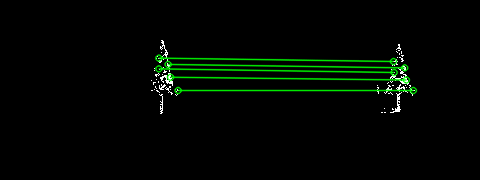
\includegraphics[width=0.9\linewidth]{images/matching.png}
    \caption{Wynik dopasowywania cech. Widoczne są dwa kolejno zarejestrowane obrazy binarne, zawierające jedną z wykrytych przeszkód. Dla par punktów w~następnym etapie przeprowadzana jest triangulacja.}
    \label{fig:matching}
\end{figure}

% Triangulacja
Dla każdej z uzyskanych par punktów przeprowadzana jest triangulacja i otrzymywane są odległości. Jako wartość dystansu do przeszkody przyjmowana jest najmniejsza z nich.

% Obliczenie składowej prędkości w kierunku drona

Dysponując wartościami odległości drona do przeszkody w~kolejnych iteracjach, łatwo obliczyć składową prędkości obiektu w~kierunku drona (prędkość względem drona) (\ref{vel}). Odejmując najnowszą i~poprzednią wartość dystansu drona do danej przeszkody, otrzymuje się zmianę jej położenia, którą w~celu otrzymania prędkości należy podzielić przez czas, w~jakim ta zmiana nastąpiła -- czyli różnicę czasów zarejestrowania przeszkody.
\begin{align}
    v_d = \frac{d_{prev} - d}{t - t_{prev}} \label{vel}
\end{align}

\noindent gdzie:
\begin{itemize}
    \item $d_{prev}$ i $d$, to odpowiednio poprzednia i obecna wartość odległości do przeszkody,
    \item $t_{prev}$ i $t$, to odpowiednio poprzednia i obecna wartość czasu zarejestrowania przeszkody.
\end{itemize}

% Ech, niechcący popsułem, przeniosłem wyniki do nowego rozdziału, a komentarze zostały tutaj - i tak wszystkie były poprawione